\documentclass[nobib]{tufte-handout}

%\\geometry{showframe}% for debugging purposes -- displays the margins

\newcommand{\bra}[1]{\left(#1\right)}
\usepackage{clrscode3e}
\usepackage{hyperref}
\usepackage[activate={true,nocompatibility},final,tracking=true,kerning=true,spacing=true,factor=1100,stretch=10,shrink=10]{microtype}
\usepackage{color}

% Fixes captions and images being cut off
\usepackage{marginfix}

\usepackage{tikz}
\usepackage{amsmath,amsthm}
\usetikzlibrary{shapes}
\usetikzlibrary{positioning}

% Set up the images/graphics package
\usepackage{graphicx}
\setkeys{Gin}{width=\linewidth,totalheight=\textheight,keepaspectratio}
\graphicspath{{.}}

\title{Notes for PHYS 27200 - Electric And Magnetic Interactions}
\author[Ezekiel Ulrich]{Ezekiel Ulrich}
\date{\today}  % if the \date{} command is left out, the current date will be used

% The following package makes prettier tables.  We're all about the bling!
\usepackage{booktabs}

% The units package provides nice, non-stacked fractions and better spacing
% for units.
\usepackage{units}

% The fancyvrb package lets us customize the formatting of verbatim
% environments.  We use a slightly smaller font.
\usepackage{fancyvrb}
\fvset{fontsize=\normalsize}

% Small sections of multiple columns
\usepackage{multicol}

% These commands are used to pretty-print LaTeX commands
\newcommand{\doccmd}[1]{\texttt{\textbackslash#1}}% command name -- adds backslash automatically
\newcommand{\docopt}[1]{\ensuremath{\langle}\textrm{\textit{#1}}\ensuremath{\rangle}}% optional command argument
\newcommand{\docarg}[1]{\textrm{\textit{#1}}}% (required) command argument
\newenvironment{docspec}{\begin{quote}\noindent}{\end{quote}}% command specification environment
\newcommand{\docenv}[1]{\textsf{#1}}% environment name
\newcommand{\docpkg}[1]{\texttt{#1}}% package name
\newcommand{\doccls}[1]{\texttt{#1}}% document class name
\newcommand{\docclsopt}[1]{\texttt{#1}}% document class option name

% Define a custom command for definitions
\newcommand{\defn}[2]{\noindent\textbf{#1}:\ #2}

\begin{document}

\maketitle

\begin{abstract}
These are lecture notes for fall 2023 PHYS 27200 at Purdue. Modify, use, and distribute as you please.
\end{abstract}

\tableofcontents

\section{Course Introduction}

This is a calculus-based physics course using concepts of electric and magnetic fields and an atomic description of
matter to describe polarization, fields produced by charge distributions, potential, electrical circuits,
magnetic forces, induction, and related topics, leading to Maxwell's equations and electromagnetic
radiation and an introduction to waves and interference. 3-D graphical simulations and numerical problem
solving by computer are employed throughout. For more information, consult the syllabus.

\section{Equations}

\begin{enumerate}
    \item Coulomb's Law: $\vec{F} = \frac{1}{4\pi \epsilon_0}\frac{q_1 q_2}{r^2}\hat{r}$
    \item Electric field due to a point or charged sphere: $\vec{E_1} = \frac{1}{4\pi \epsilon_0}\frac{q_1}{r^2}\hat{r}$
    \item Force due to electric field: $\vec{F_2} = E_1 q_2$
    \item Dipole moment between charges $-q$ and $q$ separated by $\vec{s}$: $\vec{p} = q\vec{s}$
    \item Electric field on dipole axis: $\frac{1}{4\pi \epsilon_0}\frac{-2sq}{r^3}\hat{p}$
    \item Electric field on dipole bisecting plane: $\frac{-1}{4 \pi \epsilon_0}\frac{sq}{r^3}\hat{p}$
    \item Electric field from point charge-induced dipole: $\left(\frac{1}{4\pi \epsilon_0}\right)^2 \frac{2 \alpha q_1}{r^5}\hat{r}$
    \item Electric field from dipole-induced dipole: $\left(\frac{1}{4\pi \epsilon_0}\right)^2 \frac{12 \alpha p_1^2}{r^7}$
    \item Drift speed: $\bar{v} = uE$
    \item Electric field of a uniformly charged thin rod at a distance $r$ from the midpoint,
    perpindicular to the rod: $\frac{1}{4 \pi \epsilon_0}\left[\frac{Q}{r\sqrt{r^2+(L/2)^2}}\right]$
    \item Electric field due to a charged ring, along the axis of the ring:
    $\frac{1}{4 \pi \epsilon_0}\frac{xQ}{\left(x^{2}+r_{1}^{2}\right)^{\frac{3}{2}}}$
    \item Electric field due to a charged disk, along the axis of the disk:
    $\frac{1}{2 \epsilon_0}\left(\frac{Q}{\pi r_{1}^{2}}\right)x\left(\frac{1}{x}-\frac{1}{\sqrt{r_{1}^{2}+x^{2}}}\right)$
\end{enumerate}

\pagebreak

\section{Electric charge}

\defn{Electric Charge}{Electric charge is an intrinsic characteristic of the
fundamental particles that make up objects.}

\marginnote{It was mentioned in class that mass is likewise intrinsic. 
However, when discussing the Higgs field's role in giving particles mass, 
the distinction between mass as an intrinsic or emergent property becomes 
more nuanced. The mass of elementary particles like electrons and quarks is 
emergent in the sense that it arises from their interaction with the Higgs 
field, which itself is a fundamental aspect of the universe.}

\defn{Conservation of charge}{The net charge of a \emph{closed system} never changes}

Objects can have negative, zero, or postive charge. 
Charges are always multiples of the \emph{elementary charge} $e = 1.60217662(63) \times 10^{-19} C$

\defn{Coulomb (C)}{One coulomb is the amount of charge that is
transferred through the cross section of a wire in 1 second
when there is a current of 1 ampere in the wire.}

The charges of elementary particles are listed below.
\begin{table}[ht]
    \centering
    \begin{tabular}{@{}ll@{}}
    \toprule
    Particle & Charge (elementary charge, $e$) \\
    \midrule
    Electron ($e^-$) & $-1$ \\
    Positron ($e^+$) & $+1$ \\
    Proton ($p^+$) & $+1$ \\
    Anti-proton ($p^-$) & $-1$ \\
    Neutron& $0$ \\
    Anti-neutron & $0$ \\
    Photon& $0$ \\
    \bottomrule
    \end{tabular}
    \end{table}

\defn{Point Charge}{A charged object whose
radius is much smaller than the distance
between itself and all other objects of
interest.}

The magnitude of electric force between two point charges is d
irectly proportional to the magnitude of each charge and 
inversely proportional to the distance squared. Specifically:
\[F = \frac{1}{4\pi \epsilon_0}\frac{q_1 q_2}{r^2}\]
This is Coulomb's Law. Note the direction of the force changes
with the sign of the charges involved. Like repels like and opposites
attract. 

\section{Electric field}

\begin{marginfigure}
    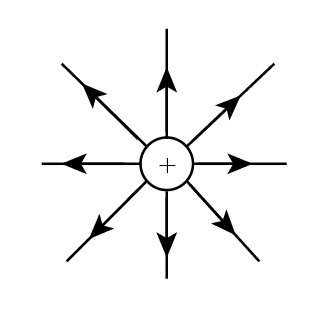
\includegraphics{images/electricfieldlines.jpg}
    \caption{An eletric field coming from point charge. 
    Notice how the densities of the lines vary with distance from the source.}
    \label{fig:electric-field-lines-point-charge}
\end{marginfigure}
Consider a charged particle. We can represent its effect
by drawing vectors that show the path a positively charged 
particle would follow if placed within its influence. These lines represent the 
electric field of the charged particle. The greater the density of the lines, the greater 
the strength of the electric field. Note that at the origin, the force is
undefined (infinite), since $|r| = 0$. 

There are many types of fields, which can be either scalar 
or vector. 
\marginnote{Technically, fields can be the more general tensor,
or even the fascinating and exotic spinor!}
For example, a temperature map is a scalar field, since
each point is associated with a scalar (the temperature at that 
point). A map of fluid velocity is a vector field, since each point 
is associated with a vector (the velocity of the fluid at that point).
For a particle, the eletric field vector at any point is given by
\[\vec{E_1} = \frac{1}{4\pi \epsilon_0}\frac{q_1}{r^2}\hat{r}\]
The direction in which the field lines point depends on the 
sign of the charge. If the charge is negative, the field lines point in.
If it is positive, the field lines point out. A useful mnemonic is
to think of the charge as someone's STD test results. If it's negative,
others will go for them and the lines point in. If it's positive, everyone
will try to get away and the lines point out.

Consider the relative strengths of the electric and 
gravitational fields. The gravitational force is given by
$F_g = G\frac{m_1m_2}{r^2}\hat{r}$, with $m_{electron} = 9 \times 10^{-31} kg$
and $m_{proton} = 1.7 \times 10^{-27} kg$. If we consider a hydrogen atom,  
then $r = 5.3 \times 10^{-11} m$. With $G = 6.7 \times 10^{-11}$, we have 
\[F_g = \frac{(1.7 \times 10^{-27})(9 \times 10^{-31})(6.7 \times 10^{-11})}{(5.3 \times 10^{-11})^2} \approx O(10^{-46})N\]
Now, the eletric force is given by $\vec{F} = \frac{1}{4\pi \epsilon_0}\frac{q_1 q_2}{r^2}\hat{r}$. 
The charge of a proton and eletric are $q_1 \approx q_2 \approx 1.6 \times 10^{-19} C$.
Ergo, since $\frac{1}{4\pi \epsilon_0} \approx 8.99 \times 10^9 \frac{Nm^2}{C^2}$, 
\[F_e = \frac{(8.99 \times 10^9 \frac{Nm^2}{C^2})(1.60\times10^{-19}C)^2}{(5.3\times10^{-11}m)^2} \approx O(10^-17)N\]
This means that $\frac{F_e}{F_g}\approx 2.27 \times 10^{39}$, meaning the eletric force is
much stronger for these masses and charges than gravity. On scales as large as humans and planets,
gravity is the dominant force because gravity is strictly additive.

For sufficient distances, the eletric field
of a uniformly charged spherical shell resembles
the eletric field of a point charge. 

\begin{marginfigure}
    \begin{center}
    \begin{tikzpicture}
        % Dot
        \fill (0,0) circle (1pt);
        % Arrow
        \draw[->] (0,0) -- (0,3);
    \end{tikzpicture}
    \end{center}

    \caption{Notice how a circle resembles a point from a great distance.}
    \label{fig:long-distance-point-sphere}
\end{marginfigure}

That means for $r>>R$, $\vec{E_{sphere}} = \frac{1}{4\pi \epsilon_0}\frac{q_1}{r^2}\hat{r}$
This holds only for outside the sphere. Inside, it can be shown that the electric field is zero. 

\defn{Superposition Principle}{The net electric field at a location in space is a
vector sum of the individual electric fields contributed by all
charged particles located elsewhere.}

To introduce systems with multiple sources of electric field lines, consider
the particle pair known as a dipole. Dipoles consist of one negatively charged
and one positively charged particle, like so:
\begin{marginfigure}
    \centering
    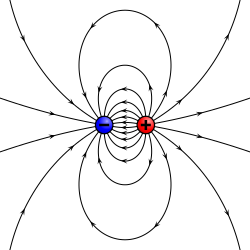
\includegraphics[width=\textwidth / 2]{images/VFPt_dipole_electric.svg.png}
    \caption{Two oppositely charged particles distanced from one another}
    \label{fig:dipole}
\end{marginfigure}

\defn{Dipole Moment}{The dipole moment is a way of expressing asymmetrical charge distribution.
It is a vector quantity, i.e. it has magnitude as well as definite directions.} The
dipole moment is given by the expression $\vec{p} = q\vec{d}$, where $q$ is
the charge on one end of the dipole and $\vec{d}$ is the distance between dipoles.

On the axis of the dipole (i.e. the lines
formed by the two particles), the electric field is 
\[\vec{E} = \frac{1}{4\pi \epsilon_0}\frac{2sq}{r^3}\hat{p}\]
where $r$ is the distance from the point in consideration to the
center of the dipole.
On the bisecting plane (i.e., the plane exactly halfway from each 
point) the field is given by
\[\vec{E} = \frac{-1}{4 \pi \epsilon_0}\frac{sq}{r^3}\hat{p}\]
Where $r$ is the distance from the point to either dipole.
The force on a positive point charge $q_1$ a 
distance of $d$ away from the dipole, aligned with the dipole, and 
on the side of the negative charge is given by 
\[\vec{F}=q_1\vec{E_{dipole}}=q_1(\frac{-1}{4\pi \epsilon_0}\frac{2qs}{d^3},0,0)\]
Note that the field will be parallel to the axis of the dipole: this 
can simplfy vector calculations.
Now consider a dipole in a uniform electric field, like so:
\begin{figure}
    \caption{Dipole in uniform electric field}
    \center
    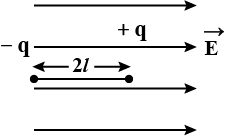
\includegraphics[width=\textwidth /2]{images/dipoleinuniformelectricfield.png}
\end{figure}
The positive end will be pulled to the right and the negative 
end to the left, exerting a torque given by $\vec{\tau} = \vec{p} \times \vec{E_{uniform}}$.
Note that by the definition of $\times$, $\tau = p E_{uniform} \sin{\theta}$, where $\theta$ is the
dipole's angle from horizontal. It can be shown that the potential
energy of a dipole in a uniform eletric field is $U = -\vec{p} \cdot \vec{E_{uniform}}$
and similarly as before (but now with $\cdot$) $U = -p E_{uniform} \cos{\theta}$. Usefully,
this means dipoles can be used to measure the direction of an electric field. 

Throughout these examples, we have been assuming the associated 
speeds are much less than the speed of light. If the velocities
approach a significant fraction of the speed of light Coulomb's
law no longer holds, and we must account for relativity. 

\defn{Conservation of Charge}{Charge cannot be created nor 
destroyed, with the exception of electron-positron annihilation
and other such quantum hijinks.} We can use conservation
of charge to predict the behavior 
\marginnote{Interestingly, in annihilation
between positrons and electrons (or any other 
subatomic particles) the total energy and momentum 
of the initial pair are conserved in the process and 
distributed among a set of other particles in the final state
(photons in the example of the electron-positron pair). 
Antiparticles have exactly opposite additive quantum numbers 
from particles, so the sums of all quantum numbers of 
such an original pair are zero. Hence any set of 
particles may be produced whose total quantum numbers are 
also zero as long as conservation of energy, 
conservation of momentum, and conservation of spin are obeyed.}
of many systems. For example, consider tape pulled from a roll.
You may have noticed when dangling strips of freshly-pulled tape 
they tend to drift towards nearby surfaces to stick and become tangled:
this is because peeling a strip of tape off a roll strips electrons 
from the tape, resulting in a net positive charge because of 
conservation of charge. When this charge approaches a net neutral 
object, such as your hand, the electrons in the atoms of your hand
are attracted to the positively charged tape and congregate closer to the tape.
This results in a negative charge buildup near the tape. The
positive tape is attracted to the negative charges, and so the tape
moves towards your hand and becomes tangled and useless. The process
of one charge inducing a charge on a neutral object occurs 
often enough for the phenomenon to be named. We call it
\defn{Polarization}{The process by which a dipole is formed
in a neutral object by an electric field.} The dipole moment is given by
$\vec{p} = \alpha \vec{E}$, where $\alpha$ is a material-dependent constant
called polarizability. Such a dipole is \emph{induced}. Consider 
a point charge near a neutral atom. The point charge creates an 
electric field given by 
\[\vec{E_1} = \frac{1}{4\pi \epsilon_0}\frac{q_1}{r^2}\hat{r}\]
Inducing a dipole given by the expression
\[\vec{p} = \alpha \vec{E_1} = \frac{1}{4\pi \epsilon_0}\frac{\alpha q_1}{r^2}\hat{r}\]
This dipole creates a field at the point charge of
\begin{align*}
    \vec{E_2} &= \frac{1}{4\pi \epsilon_0}\frac{2\vec{p}}{r^3} \\
    &= \frac{1}{4\pi \epsilon_0}\frac{2\alpha \vec{E_1}}{r^3} \\
    &= \frac{1}{4\pi \epsilon_0}\frac{2\alpha}{r^3}(\frac{1}{4\pi \epsilon_0} \frac{q_1}{r^2}\hat{r}) \\
    &= \left(\frac{1}{4\pi \epsilon_0}\right)^2 \frac{2 \alpha q_1}{r^5}\hat{r}
\end{align*}
This formula is valid provided the electric field that induced the dipole is 
from a point charge. If the electric field is instead from, say, another (permanent)
dipole then $\vec{p} = \alpha \vec{E_1}$ is still valid. However, in this case
the formula for $\vec{E_1}$ will be given by the equation for the electric field
along the axis of a dipole instead. Following this logic, 
\begin{align*}
    \vec{p} &= \alpha \vec{E_1} \\
    &= \alpha \frac{1}{4\pi \epsilon_0}\frac{2\vec{p_1}}{r^3} \\
\end{align*}
If we let $\vec{r'}$ be the location of the permanent dipole from the induced 
dipole, we have the electric field at the permanent dipole as 
\begin{align*}  
    \vec{E}(\vec{r'}) &= \left(\frac{1}{4\pi \epsilon_0}\frac{2}{r^3}\right)\left(\alpha \frac{1}{4\pi \epsilon_0}\frac{2\vec{p_1}}{r'^3}\right) \\
    &= \left(\frac{1}{4\pi \epsilon_0}\right)^2 \frac{4 \alpha \vec{p_1}}{r^3 r'^3}\\
\end{align*}
Calculating the force on the permanent dipole is slightly more complicated than
multiplying by the charge of the dipole, since $r'$ and the sign of 
$q$ varies based on which end of the dipole we consider. To find the net force, we
must find the force on each charge and sum them, like so:
\begin{align*}  
    F^+ &= q\vec{E}(r - \frac{s}{2}) \\
    F^- &= q\vec{E}(r + \frac{s}{2}) \\
    F_{net} &= F^+ + F^- \\
    &= q\left[\left(\frac{1}{4\pi \epsilon_0}\right)^2 \frac{4 \alpha \vec{p_1}}{r^3 (r + \frac{s}{2})^3} - \left(\frac{1}{4\pi \epsilon_0}\right)^2 \frac{4 \alpha \vec{p_1}}{r^3 (r - \frac{s}{2})^3}\right] \\
    &= q\left(\frac{1}{4\pi \epsilon_0}\right)^2 \left[\frac{4 \alpha \vec{p_1}}{r^3 (r + \frac{s}{2})^3} - \frac{4 \alpha \vec{p_1}}{r^3 (r - \frac{s}{2})^3}\right] \\
    &= q\left(\frac{1}{4\pi \epsilon_0}\right)^2\left(4 \alpha \vec{p_1}\right) \left[\frac{1}{r^3 (r + \frac{s}{2})^3} - \frac{1}{r^3 (r - \frac{s}{2})^3}\right] \\
\end{align*}
With a bit more algebraic simplification and the assumption
that $r >> s$, we can show that
\begin{align*}  
    F_{net} &= F^+ + F^- \\
    &= q\left(\frac{1}{4\pi \epsilon_0}\right)^2 \left(\frac{4 \alpha \vec{p_1}}{r^6}\right) \left[(1+\frac{3s}{2r})-(1-\frac{3s}{2r})\right]\\
    &= q\left(\frac{1}{4\pi \epsilon_0}\right)^2 \left(\frac{4 \alpha \vec{p_1}}{r^6}\right) \left[\frac{3s}{r}\right]\\
    &\approx q\left(\frac{1}{4\pi \epsilon_0}\right)^2 \left(\frac{12 \alpha \vec{p_1}s}{r^7}\right) \\
    &= \left(\frac{1}{4\pi \epsilon_0}\right)^2 \frac{12 \alpha p_1^2}{r^7}
\end{align*}

\section{Insulators, conductors, and Van der Waals forces}

On the topic of induced dipoles, consider how freely moving
atoms in a substance interact. The electrons are dispersed 
in a cloud about the nucleus of each atom. These clouds can be thought 
of as constantly fluctuating, and occasionally these fluctuations 
will result in more electrons on one side than another. In this 
case there will be a small dipole. If this dipole approaches another
atom (which may or may not have its own temporary dipole) the two will
be attracted. The result of this interaction is that even neutral 
materials can be attracted to each other due to the fluctuating 
dipoles of its electron clouds. We call this phenomenon

\defn{Van der Waals forces}{attraction and repulsions 
between atoms, molecules, as well as other intermolecular 
forces. Caused by correlations in the 
fluctuating polarizations of nearby particles 
(a consequence of quantum dynamics)}.
\begin{marginfigure}
    \caption{Effect of electric field on insulator}
    \center
    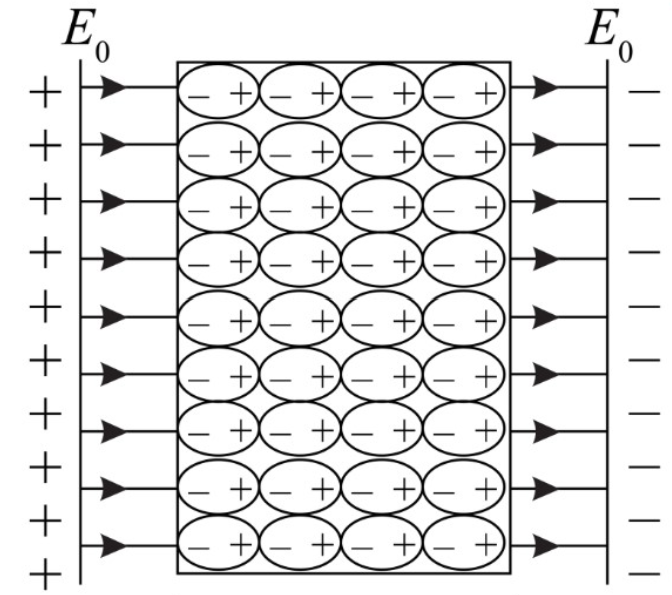
\includegraphics[width=\textwidth/2]{images/insulator.png}
    \label{fig:insulator}
\end{marginfigure}
\defn{Insulator}{An insulator is a material that does not 
easily allow electricity to pass through it}. Inside
an insulator the electrons are bound to their atoms, but they
may still shift in response to an electric field (see fig. \ref{fig:insulator})
This results in the insulator becoming polarized. 
Just as with most polarized objects, we can approximate 
its dipole moment with $\vec{p} = \alpha \vec{E}$
This relationship is only valid if the electrons 
are bound to the stationary constituent atoms. 
If this is not the case, then the a material in 
question is called a

\defn{Conductor}{A conductor is a material 
that allows electricity to flow freely through it}. 
For example, consider a liquid with charged atoms floating
throughout.
\marginnote{Such a liquid is called an \emph{ionic solution}}
Here, when an electric field is applied,
the charges each follow the electric field lines
until they reach the edges of whatever container holds them. 
%show that the electric field within is zero
More commonly, we see conductors in the form of metals. 
The atomic structure of a metal allows electrons to move freely
from atom to atom. Thus, within a metal, the electrons can freely 
move in whichever direction the electric field determines.
\marginnote{Typically electrons are bound to the metal as a whole. However,
if the electric field is strong enough, then air surrounding
a metal can become ionized and allow electrons to flow freely
through it, creating a spark.}
"Freely" is used liberally here, since the electrons 
can collide with other electrons or defects in the metal and lose energy.
The mobile electrons in 
the conductor will have a momentum and velocity given by 
\begin{align*}
    \vec{\Delta p} &= \vec{F_{net}} \Delta t \\
    &= q\vec{E_{net}} \\
    &= -e \vec{E_{net}} \\
    &\rightarrow \vec{\Delta p} = -e \vec{E_{net}} \Delta t \\
    &= m_e v \\
    &\rightarrow v = \frac{e \vec{E_{net}} \Delta t}{m_e}\\
\end{align*}
A good approximation for the average velocity of 
an electron is $\bar{v} = \mu E$. The constant $\mu$ is called
the "mobility". 

Now, consider a conductor with a net charge, such as a charged sphere.
Inside the sphere like charges will repel each another and push 
to get as far away from one another as possible. This occurs when
all the charges are on the surface of the conducting object, since anywhere 
else would be closer together and they cannot go outside the 
bounds of the object. This rearrangement has two effects.
First, any charge in a conductor will be found on the surface.
Second, the net electric field inside a conductor will be zero. 
\marginnote{To see why this must be the case, imagine if it 
were not. Then any charge within the conductor would be moved
by the electric field, so we see that the case where no electric field
is present is the only stable possibility. However, if electrons 
are moving, then there can be (and is) an electric field within
the conductor. It is only when the conductor is in static 
equilibrium that there is no net electric field within.}
An interesting result of electrons seeking to minimize repulsion inside a conductor is 
the \emph{sharp point effect}. To visualize this effect, imagine a gymnasium full of students 
pretending to be electrons, staying as far away from others as possible. 
Anyone near the center of the crowd will feel badly pressed and will try 
to work there way towards the edge of the gym, where at least one side 
will no longer have fellow students milling about. The result? 
Most of the students will gravitate towards the edge of the gym 
and hover there, to take advantage of that lack of other students 
on the wall side of the gym. Now imagine a narrow corridor leading out of the gym. 
Even better! Students in that corridor will only have 
fellow students behind and in front of them.
Now imagine the very end of that corridor, a sort of point. 
Even better! Now, the student who finds that spot will benefit 
from having only one student nearby. But somewhat ironically, 
that same effect will cause other students to pack themselves 
into the long, narrow corridor more tightly, since pretty 
much anywhere in the corridor makes them less exposed to the 
full set of students than being in the gym does.
This effect makes edges, wires, and points more attractive to electrons, 
which similarly just don't want other electrons nearby.

\section{Finding electric field}

Now that we understand conceptually how charge behaves in a conductor, 
let's think about the electric field that charge creates. We can
visualize any charged object as a collection of point charges in the shape of 
the object. If we'd like to find the net electric field of these charges, 
we simply use Coulomb's law and sum up each of their electric fields. To 
illustrate this approach, imagine a charged rod with length $L$ and charge $Q$. We can 
approximate it as a bunch of charges in a row. For now, let's use ten, but
recognize that the more charges we use the better our estimate will be. 
Each piece of the rod will have a charge of $\frac{Q}{10}$, so to find 
the electric field at a point we would need to calculate the vector between each piece 
and the point and use $\vec{F} = \frac{1}{4\pi \epsilon_0}\frac{q_1 q_2}{r^2}\hat{r}$. 
We would do this ten times and then sum the electric fields to get our approximate net field. 
Of course, perhaps we would like to find the exact electric field. To do this
we would have to cut our object up into an infinite number of points, find the 
infinitesimal electric field due to each, and sum them up. Sound familiar? 

To drive the point home, consider a vertical rod with a uniform charge of $Q$ and length $L$. 
Let's take a point on the bisecting plane of this rod (the horizontal plane that cuts the rod in half).
Say we view this point from the side and see that is has coordinates $(0, x)$. 
If we want to find the electric field due to a little bit of the rod at $\vec{x}$, 
we need to know the distance between them. If the bit is a distance of $y$ up the rod,
the distance between it and $\vec{x}$ will be $r = \sqrt{x^2 + y^2}$. 
The charge of this small piece will be $\frac{Q}{L} \Delta y$ (where $\Delta y$ is the 
height of the peice), and $\hat{r}$ 
will be $\frac{(x,-y)}{\sqrt{x^2+y^2}}$. 
Therefore the electric field at $\vec{x}$ will be given by 
\begin{align*}
    \Delta \vec{E} &= \frac{1}{4\pi \epsilon_0}\frac{q_1}{r^2}\hat{r} \\
    &= \frac{1}{4\pi \epsilon_0}\frac{\frac{Q}{L} \Delta y}{x^2+y^2}\frac{(x,-y)}{\sqrt{x^2+y^2}}
\end{align*}
We can see by symmetry (isn't symmetry lovely?) that the contributions in the $y$
direction will cancel, so we need only consider the $x$ direction. Therefore, 
\begin{align*}
    \Delta \vec{E} &= \frac{1}{4\pi \epsilon_0}\frac{\frac{Q}{L} \Delta y}{x^2+y^2}\frac{x}{\sqrt{x^2+y^2}} \\
    &= \frac{Q}{4\pi \epsilon_0 L}\frac{x \Delta y}{(x^2+y^2)^{3/2}}
\end{align*}
Now comes the tricky part: adding these up. You have already likely guessed that
we will need to integrate between the bottom and top of the rod, which
corresponds to the integral from $-\frac{L}{2}$ to $\frac{L}{2}$. We have then
\begin{align*}
    \vec{E} &= \int_{-L/2}^{L/2} \frac{Q}{4\pi \epsilon_0 L}\frac{x}{(x^2+y^2)^{3/2}} dy\\
\end{align*}
I'll spare you the tedious integration and skip to the result:
\begin{align*}
    \vec{E} &= \frac{1}{4 \pi \epsilon_0}\left[\frac{Q}{x\sqrt{x^2+(L/2)^2}}\right]\hat{x}\\
\end{align*}

The steps for finding the electric field due to a charged object in general are outlined below.
\begin{enumerate}
    \item Cut up the charge distribution into pieces and draw $\Delta \vec{E}$
    \begin{itemize}
        \item Divide the charge distribution into pieces whose field is known. 
        In particular, very small pieces can be approximated by point particles.
        You may also wish to break up a complex object into smaller objects whose
        electric field equations are already known. 
        \item Pick a representative piece, and at the location of interest draw a 
        vector $\Delta \vec{E}$ showing the contribution to the electric field of this representative piece. 
        Drawing this vector helps you figure out the direction of the net field at the location of interest.
    \end{itemize}
    \item Write an expression for the electric field due to one piece
    \begin{itemize}
        \item Pick an origin for your coordinate system, and show it on your diagram.
        Draw the vector $\vec{r}$ from the source piece to the observation location. 
        Write algebraic expressions for $\vec{r}$ and $\hat{r}$.
        \item Write an algebraic expression for the magnitude $|\Delta \vec{E}|$ contributed by the representative piece. Multiply by
        $\hat{r}$ to get the vector $\Delta \vec{E}$. You can break this up into 
        $x$, $y$, and $z$ components for integration. Once you do each expression should 
        contain one or more “integration variables” ($\Delta x/\Delta y/ \Delta z$ or $dx/dy/dz$) related to the coordinates of the piece.
        Write the amount of charge on the piece, $\Delta q$, in terms of your variables. 
    \end{itemize}
    \item Sum the contributions of all the pieces
    \begin{itemize}
        \item The net field is the sum of the contributions of all the pieces. 
        To write the sum as a definite integral, you must include limits 
        given by the range of the integration variable. If the integral 
        can be done symbolically, do it. If not, choose a finite number 
        of pieces and do the sum with a calculator or a computer.
    \end{itemize}
    \item Check the result
    \begin{itemize}
        \item Check that the direction of the net field is qualitatively correct.
        \item Check the units of your result, which should be newtons per coulomb.
        \item Look at special cases. For example, if the net charge is 
        nonzero, your result should reduce to the field of a point 
        charge when you are very far away. For a numerical integration 
        on a computer, check that the computation gives the correct numerical 
        result for special cases that can be calculated by hand.
    \end{itemize}
\end{enumerate}

Let's apply these steps to some new problems. First, let's consider the electric field
produced by a charged ring (fig. \ref{fig:ring}).
\begin{figure}
    \center
    \caption{Charged ring}
    \label{fig:ring}
    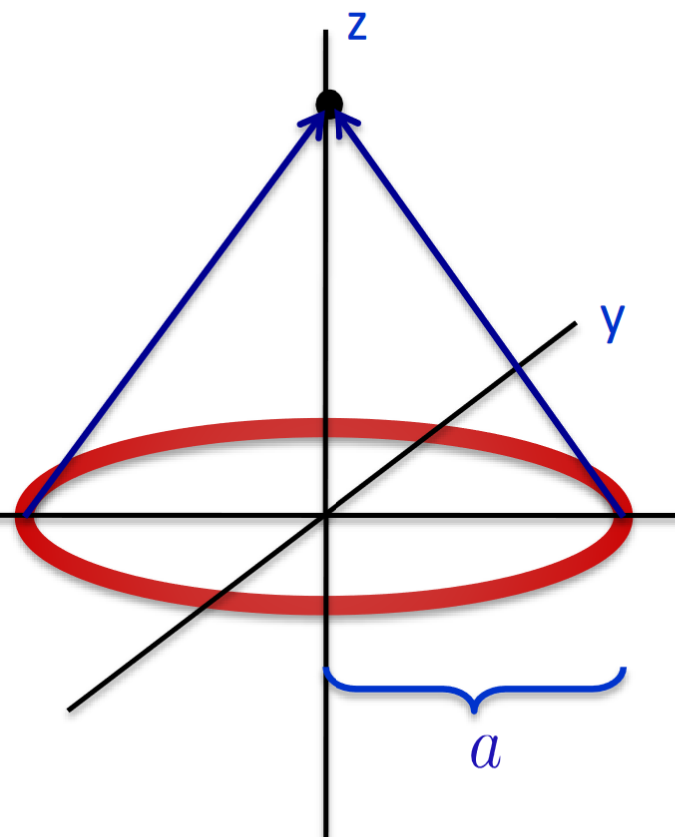
\includegraphics[width=\textwidth/2]{images/ring.png}
\end{figure}
We have a ring of radius $a$, with a charge of $Q$. The ring is centered on the xy plane
and we are calculating the electric field on the z-axis. 
\begin{enumerate}
    \item Cut the charge distribution and find $\Delta \vec{E}$. 
    \begin{figure}
        \center
        \caption{Charged ring slice}
        \label{fig:ringslice}
        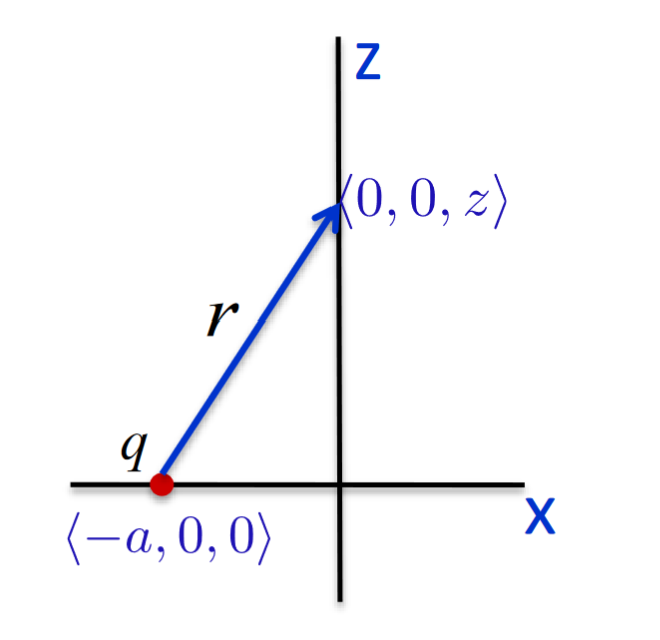
\includegraphics[width=\textwidth/2]{images/ringslice.png}
    \end{figure}
    Let's take a slice of this ring, like fig. \ref{fig:ringslice}. We can 
    view the slice of the annulus here as a point charge a distance 
    of $\sqrt{a^2+z^2}$ away from $(0,0,a)$. We find then that 
    \begin{align*}
        \vec{r} &= (a,0,z) \\
        \hat{r} &= \frac{(a,0,z)}{\sqrt{a^2+z^2}}
    \end{align*}
    %what is \Delta e?
    \item By symmetry, only the z components of each individual electric field
    contribute. Therefore, 
    \begin{align*}
        \vec{E} &= \sum \frac{1}{4 \pi \epsilon_0} \frac{z \Delta q}{(a^2+z^2)^{3/2}}
    \end{align*}
    \item Since the charge is uniformly distributed, we have that 
    $\Delta q = \frac{Q \Delta \theta}{2 \pi}$. 
    Therefore our integral becomes 
    \begin{align*}
        \vec{E} &= \int_0^{2 \pi} \frac{1}{4 \pi \epsilon_0} \frac{z \frac{Q}{2 \pi}}{(a^2+z^2)^{3/2}} d \theta \\
        &= \frac{Q}{4 {\pi}^2 \epsilon_0}\frac{z}{{(a^2+z^2)^{3/2}}} \int_{0}^{2\pi}d\theta \\
        &= \frac{1}{4 \pi \epsilon_0}\frac{Qz}{{(a^2+z^2)^{3/2}}}\hat{z}
    \end{align*}
    \item This looks pretty good. It goes to zero as z goes to either zero or infinity, as it should. 
\end{enumerate}
Let's consider the electric field on the z-axis of a disk with radius $r$ and charge $Q$ now. 
\begin{enumerate}
    \item Take some point on the disk. The calculation for the electric field due to 
    this point is identical to the case of the ring. Therefore 
    \begin{align*}
        \vec{r} &= (a,0,z) \\
        \hat{r} &= \frac{(r,0,z)}{\sqrt{a^2+z^2}}
    \end{align*}
    \item Now we have that $\Delta q = \frac{Q}{\pi r^2} da d\theta$. Therefore
    \begin{align*}
        \vec{E} &= \sum \frac{1}{4 \pi \epsilon_0}\frac{z \Delta q}{(a^2+z^2)^{3/2}} \\
        &= \sum \frac{1}{4 \pi \epsilon_0} \frac{Q}{\pi r^2} \frac{z da d\theta}{(a^2+z^2)^{3/2}}
    \end{align*}
    \item 
    \begin{align*}
        \vec{E} &= \frac{1}{4 \pi \epsilon_0} \frac{Qz}{\pi r^2} \int \int \frac{a}{(a^2+z^2)^{3/2}} da d \theta \\
        &= \frac{1}{4 \pi \epsilon_0} \frac{Qz}{\pi r^2} \int_{0}^{2 \pi} \int_0^{r} \frac{a}{(a^2+z^2)^{3/2}} da d \theta \\
        &= \frac{1}{2 \epsilon_0} \frac{Qz}{\pi r^2} \left[\frac{1}{z} - \frac{1}{\sqrt{r^2 + z^2}}\right] \hat{z}
    \end{align*}
\end{enumerate}
\end{document}
